% Template for PLoS
% Version 3.1 February 2015
%
% To compile to pdf, run:
% latex plos.template
% bibtex plos.template
% latex plos.template
% latex plos.template
% dvipdf plos.template
%
% % % % % % % % % % % % % % % % % % % % % %
%
% -- IMPORTANT NOTE
%
% This template contains comments intended 
% to minimize problems and delays during our production 
% process. Please follow the template instructions
% whenever possible.
%
% % % % % % % % % % % % % % % % % % % % % % % 
%
% Once your paper is accepted for publication, 
% PLEASE REMOVE ALL TRACKED CHANGES in this file and leave only
% the final text of your manuscript.
%
% There are no restrictions on package use within the LaTeX files except that 
% no packages listed in the template may be deleted.
%
% Please do not include colors or graphics in the text.
%
% Please do not create a heading level below \subsection. For 3rd level headings, use \paragraph{}.
%
% % % % % % % % % % % % % % % % % % % % % % %
%
% -- FIGURES AND TABLES
%
% Please include tables/figure captions directly after the paragraph where they are first cited in the text.
%
% DO NOT INCLUDE GRAPHICS IN YOUR MANUSCRIPT
% - Figures should be uploaded separately from your manuscript file. 
% - Figures generated using LaTeX should be extracted and removed from the PDF before submission. 
% - Figures containing multiple panels/subfigures must be combined into one image file before submission.
% For figure citations, please use "Fig." instead of "Figure".
% See http://www.plosone.org/static/figureGuidelines for PLOS figure guidelines.
%
% Tables should be cell-based and may not contain:
% - tabs/spacing/line breaks within cells to alter layout or alignment
% - vertically-merged cells (no tabular environments within tabular environments, do not use \multirow)
% - colors, shading, or graphic objects
% See http://www.plosone.org/static/figureGuidelines#tables for table guidelines.
%
% For tables that exceed the width of the text column, use the adjustwidth environment as illustrated in the example table in text below.
%
% % % % % % % % % % % % % % % % % % % % % % % %
%
% -- EQUATIONS, MATH SYMBOLS, SUBSCRIPTS, AND SUPERSCRIPTS
%
% IMPORTANT
% Below are a few tips to help format your equations and other special characters according to our specifications. For more tips to help reduce the possibility of formatting errors during conversion, please see our LaTeX guidelines at http://www.plosone.org/static/latexGuidelines
%
% Please be sure to include all portions of an equation in the math environment.
%
% Do not include text that is not math in the math environment. For example, CO2 will be CO\textsubscript{2}.
%
% Please add line breaks to long display equations when possible in order to fit size of the column. 
%
% For inline equations, please do not include punctuation (commas, etc) within the math environment unless this is part of the equation.
%
% % % % % % % % % % % % % % % % % % % % % % % % 
%
% Please contact latex@plos.org with any questions.
%
% % % % % % % % % % % % % % % % % % % % % % % %

\documentclass[10pt,letterpaper]{article}
\usepackage[top=0.85in,left=2.75in,footskip=0.75in]{geometry}

% Use adjustwidth environment to exceed column width (see example table in text)
\usepackage{changepage}

% Use Unicode characters when possible
\usepackage[utf8]{inputenc}

% textcomp package and marvosym package for additional characters
\usepackage{textcomp,marvosym}

% fixltx2e package for \textsubscript
\usepackage{fixltx2e}

% amsmath and amssymb packages, useful for mathematical formulas and symbols
\usepackage{amsmath,amssymb}

% cite package, to clean up citations in the main text. Do not remove.
\usepackage{cite}

% Use nameref to cite supporting information files (see Supporting Information section for more info)
\usepackage{nameref,hyperref}

% line numbers
\usepackage[right]{lineno}

% ligatures disabled
\usepackage{microtype}
\DisableLigatures[f]{encoding = *, family = * }

% rotating package for sideways tables
\usepackage{rotating}

\usepackage{verbatim}   % useful for program listings

% Remove comment for double spacing
%\usepackage{setspace} 
%\doublespacing

% Text layout
\raggedright
\setlength{\parindent}{0.5cm}
\textwidth 5.25in 
\textheight 8.75in

% Bold the 'Figure #' in the caption and separate it from the title/caption with a period
% Captions will be left justified
\usepackage[aboveskip=1pt,labelfont=bf,labelsep=period,justification=raggedright,singlelinecheck=off]{caption}

% Use the PLoS provided BiBTeX style
\bibliographystyle{plos2015}

% Remove brackets from numbering in List of References
\makeatletter
\renewcommand{\@biblabel}[1]{\quad#1.}
\makeatother

% Leave date blank
\date{}

% Header and Footer with logo
\usepackage{lastpage,fancyhdr,graphicx}
\usepackage{epstopdf}
\pagestyle{myheadings}
\pagestyle{fancy}
\fancyhf{}
\lhead{
\includegraphics[width=2.0in]{PLOS-submission.eps}}
\rfoot{\thepage/\pageref{LastPage}}
\renewcommand{\footrule}{\hrule height 2pt \vspace{2mm}}
\fancyheadoffset[L]{2.25in}
\fancyfootoffset[L]{2.25in}
\lfoot{\sf PLOS}

%% Include all macros below

\newcommand{\lorem}{{\bf LOREM}}
\newcommand{\ipsum}{{\bf IPSUM}}

%% END MACROS SECTION


\begin{document}
\vspace*{0.35in}

% Title must be 250 characters or less.
% Please capitalize all terms in the title except conjunctions, prepositions, and articles.
\begin{flushleft}
{\Large
\textbf\newline{Calculating Effective Viscosity and Active Stress in a Model 2D Active Network}
}
\newline
% Insert author names, affiliations and corresponding author email (do not include titles, positions, or degrees).
\\
William McFadden\textsuperscript{1},
Edwin Munro\textsuperscript{2,*}
\\
\bigskip
\bf{1} Biophysical Sciences Program, University of Chicago, Chicago, IL, USA
\\
\bf{2} Department of Molecular Genetics and Cell Biology, University of Chicago, Chicago, IL, USA
\\
\bigskip

% Insert additional author notes using the symbols described below. Insert symbol callouts after author names as necessary.
% 
% Remove or comment out the author notes below if they aren't used.
%
% Primary Equal Contribution Note
%\Yinyang These authors contributed equally to this work.

% Additional Equal Contribution Note
% Also use this double-dagger symbol for special authorship notes, such as senior authorship.
%\ddag These authors also contributed equally to this work.

% Current address notes
%\textcurrency a Insert current address of first author with an address update
% \textcurrency b Insert current address of second author with an address update
% \textcurrency c Insert current address of third author with an address update

% Deceased author note
%\dag Deceased

% Group/Consortium Author Note
%\textpilcrow Membership list can be found in the Acknowledgments section.

% Use the asterisk to denote corresponding authorship and provide email address in note below.
* emunro@uchicago.edu

\end{flushleft}
% Please keep the abstract below 300 words
\section*{Abstract}
Lorem ipsum dolor sit amet, consectetur adipiscing elit. Curabitur eget porta erat. Morbi consectetur est vel gravida pretium. Suspendisse ut dui eu ante cursus gravida non sed sem. Nullam sapien tellus, commodo id velit id, eleifend volutpat quam. Phasellus mauris velit, dapibus finibus elementum vel, pulvinar non tellus. Nunc pellentesque pretium diam, quis maximus dolor faucibus id. Nunc convallis sodales ante, ut ullamcorper est egestas vitae. Nam sit amet enim ultrices, ultrices elit pulvinar, volutpat risus.


% Please keep the Author Summary between 150 and 200 words
% Use first person. PLOS ONE authors please skip this step. 
% Author Summary not valid for PLOS ONE submissions.   
\section*{Author Summary}
In this paper, we develop and analyze a minimal model for 2D active networks based on the cortical cytoskeleton of eukaryotic embryos.  Our model introduces the concept of active friction between cross-linked supramolecular filaments as a means to derive both macroscopic effective viscosity and active stress from microscopic properties.  We generate computational simulations based on the model, and demonstrate that active friction is sufficient to drive network contraction.  By introducing filament recycling, we are able to set up steady state flow profiles such those found in the cortex of developing embryos and migrating cells.  The model is used to calculate phenomenological constants measured in prior experiments.  Our analysis sheds insight on potential microscopic control parameters governing broad qualitative differences in 2D active networks.

\linenumbers

\section*{Introduction}

Active networks of cross-linked polymers are a class of materials with poorly understood but highly interesting properties.  Cross-linked networks of cytoskeletal polymers have been a subject of great interest to biologists  because of their importance as structural components of cells\cite{cellmech_review1,cellmech_review2}.  Furthermore, early studies of semi-flexible polymer networks reconstituted {\em in vitro} revealed novel, nonlinear rheology, spurring interest from materials scientists\cite{megareview}.  


On shorter timescales, the response of cross-linked polymer networks to applied stress can be well-described theoretically in terms of purely elastic mechanical resistance.  On longer timescales, the network's elastic resistance begins to give way to a viscous relaxation of stored stress, but the mechanisms that govern this viscous relaxation remain poorly understood.   It is important to understand the mechanism behind this long timescale relaxation of cross-linked polymer networks both for understanding their novel material properties as well as understanding how this effect may govern physiologically important cellular processes\cite{cell_rheo}.


For {\em in vitro} reconstitutions, this viscous relaxation is thought to result from transient unbinding and rebinding of intermolecular cross-links\cite{rheo_crosslinksmatter,theo_crosslinkslip1}. However, there is still no clear understanding of how local relaxations of network connectivity would give rise to a global viscous relaxation.  In our work, we wish to expand upon a well-established mechanical picture of cross-linked semi-flexible polymer networks to incorporate slippage of cross-links over longer timescales.  


\subsection*{Short Timescale Mechanics of Cross-linked Actin Filament Networks}


Early {\em in vitro}  studies of cross-linked actin filament networks revealed strikingly different elastic behaviors compared to the already well-understood flexible polymer gels \cite{rheo_bench}.  The complexity of these behaviors drove a surge in both experimental and theoretical studies of semi-flexible networks.  For a comprehensive review of this field we recommend \cite{megareview}, but we will shortly repeat some important milestones here.

\paragraph{Theories of Semi-flexible Filament Networks}
 
Diversity and discrepancy in observations led a drive toward systematic {\em in vitro} experimental explorations of the rheology of cross-linked semi-flexible polymer networks at short timescales.  In studies with rigid irreversibly cross-linked networks, it was found that differences in network structure could lead to remarkably different elastic moduli, suggesting distinct phases of mechanical response \cite{rheo_marge}.  These discoveries in turn begat theoretical work on the basic implications of the semi-flexible nature of filaments on network mechanics.  

Prior work on the basic physics of individual semi-flexible polymers \cite{mol_wlc,theo_doi_ed}, and comprehensive theories of semi-flexible filament solutions, \cite{theo_morse} laid a groundwork for theoretical considerations of cross-linked networks. Beginning with the so-called "mikado model" descriptions\cite{theo_hlm,theo_hlm2}, it was determined that there should exist a minimum rigidity percolation threshold, and that the connectivity of the network determined whether the mechanical response was dominated by non-affine bending or affine stretching of filaments.   Continuing to more explicit theories\cite{theo_best}, the mechanics of rigidly cross-linked networks were shown to be well-described in terms of purely elastic stretching of filaments between cross-linked points. 

\paragraph{Incorporating Effects of Cross-link Compliance}

Despite the success of the theory for rigid cross-links, early studies showed that surprising qualitative differences in mechanical response could be traced to differences in the chosen cross-linker\cite{rheo_crosslinkcompare,rheo_crosslinkreview}.  In addition, many studies using more compliant cross-linkers showed that cross-linker compliance could give rise to different nonlinear rheological properties on short timescales\cite{rheo_crosslink_nonlin1,rheo_crosslink_nonlin2,rheo_crosslink_nonlin3,rheo_crosslink_notactin}. Making matters even more complicated, ongoing research has begun to uncover added complexity from more highly complex issues such as filament bundling\cite{theo_crosslinkslip2,model_massive}and the effects of active cross-linking by molecular motors\cite{rheo_active}.

While theorists have built a number of largely successful models that help characterize different aspects of the cross-link dominated response\cite{theo_nonaffine2,theo_floppy,theo_crosslinknonlinear}, the diversity of behaviors of these networks makes a precise yet general theory more difficult.


\subsection*{Long Timescale Stress Relaxation from Transient Cross-link Unbinding}

At long timescales, the purely elastic behavior of cross-linked networks gives way to fluid-like stress relaxation. Additionally, fluid-like flows have been observed in a number of cellular processes\cite{cellmech_flows,cellmech_flows2,cellmech_flows3,rheo_fluid,rheo_fluid2,cell_rheo_exp}.  In {\em in vitro} studies, long timescale creep behaviors are thought to arise predominantly from the transient nature of filament binding for most biologically relevant cross-linkers\cite{rheo_crosslinkslip1,rheo_crosslinkslip2,rheo_crosslinkslip3,rheo_nonaffine}.  While the importance of cross-link dynamics in determining the mechanical response of semi-flexible polymer networks has been known for at least 20 years\cite{rheo_crosslinksmatter}, there is still a gap in our understanding of how microscopic cross-link unbinding relates to viscous flows. 

\paragraph{Models of Stress Relaxation with Transient Cross-links}

The dependence of network rheology on cross-link unbinding is an active subject of theoretical research\cite{theo_crosslinkslip2}.  

Several theoretical methods have addressed cross-link binding and unbinding directly \cite{theo_crosslinkslip1,theo_crosslinkslip2} in analytical approaches that allowed well-constrained fits for specific cross-linkers.  These theories have therefore focused conceptually at the level of the cross-linked filament and were extended analytically to macroscopic networks.  In another approach, modelers have taken cross-links as extended springlike structures \cite{model_taeyoon} that are able to bind and unbind in simulated filament networks. Finally, other more ambitious simulations have even sought to interrogate the effects of cross-link unbinding in combination with the more complex mechanics of filament bundles\cite{rheo_crosslinkslip2,theo_crosslinkslip3}.

Ultimately, the complexity of the many theoretical approaches that have been applied to this problem have made it difficult to distinguish what, if any, core physical mechanisms may be sufficient to explain the observed forms of stress relaxation.  We believe that serious qualitative understanding can be generated by focusing on some of the common elements exhibited in the aforementioned literature.

\paragraph{Novelty of Cross-link Slip Approach}

Here, we introduce a coarse-grained representation of filament cross-linking in which cross-linked filaments which are able to slide past each other as molecular bonds form and rupture, akin to coarse-grained models of molecular friction\cite{theo_friction,theo_frictionSam,theo_molefric}.  This drag-like coupling has been shown to be an adequate approximation in the case of ionic cross-linking of actin\cite{mol_fric,theo_hydroish2}, and can be found in the theoretical basis of force-velocity curves for myosin bound filaments\cite{theo_frictionShila}. We propose that it will form a suitable bulk approximation in the presence of super molecular cross-links as well.

Importantly, this simplification allows us to extend our single polymer models to dynamical systems of larger network models for direct comparison between theory and modeling results.  This level of coarse graining will therefore make it easier to understand classes of behavior for varying compositions of cross-linked filament networks.  In addition, it allows us to compute a new class of numerical simulations efficiently, which gives us concrete predictions for behaviors in widely different networks with measurable dependencies on molecular details.












% You may title this section "Methods" or "Models". 
% "Models" is not a valid title for PLoS ONE authors. However, PLoS ONE
% authors may use "Analysis" 
\section*{Models}
\subsection*{Composite Cross-link \& Filament Representation}
We consider individual filaments as chains of springs with relaxed length $l_s$.  The orientations of neighboring springs are linearly coupled. Filaments can therefore be represented as a sequence of nodes with positions $\mathbf{x_i}$ and nearest neighbor interactions of the form

\begin{equation}
|F_{i,i+1}|_{\parallel} = -\mu\cdot\frac{|\mathbf{x_{i+1}}-\mathbf{x_i}|-l_s}{l_s} 
\end{equation}

\begin{equation}
|F_{i,i+2}|_{\perp} = -\frac{\kappa}{l_s^2}\cdot acos\left (\frac{\mathbf{x_{i+2}}-\mathbf{x_{i+1}}}{|\mathbf{x_{i+2}}-\mathbf{x_{i+1}}|} \cdot\frac{\mathbf{x_{i+1}}-\mathbf{x_i}}{|\mathbf{x_{i+1}}-\mathbf{x_i}|} \right ) 
\end{equation}


where, $\mu$ represents an extensional modulus of a filament, and $\kappa$ represents a bending modulus.   This is essentially a discretized equivalent to a model of filaments with separable extensional and bending moduli as in \cite{theo_hlm}.  We define the totally elastic force on a node as

\begin{equation}
\nabla{\cal H}_i =|F_{i,i+1}|_{\parallel} + |F_{i,i+2}|_{\perp}
\end{equation}

Here, we take the extensional modulus as a composite quantities related to both filament and cross-linker compliance in a manner similar to a recently proposed effective medium theory\cite{theo_crosslinknonlinear}.  In the limit of highly rigid cross-links and flexible filaments, our model reduces to the pure semi-flexible filament models of \cite{theo_hlm,theo_hlm2}.  In the opposite regime of nearly rigid filaments and highly flexible cross links, our method is still largely similar to the model of \cite{theo_crosslinknonlinear} in small strain regimes before any nonlinear cross link stiffening.  However, in departure from those models, the magnitude of the force on interior cross-links in our model is still the same as those on the exterior.  This is a simplification of the varying levels of strain that would actually be present in these cross-linkers as addressed in \cite{theo_crosslinknonlinear}, but we choose to ignore the slight variation in favor of an approximated, global mean approach.  




\subsection*{2D Network Formation}

We choose to focus our attention on 2D networks both for their tractability as well as their relevance in the quasi-2D cytoskeletal cortex of many eukaryotic cells\cite{cellmech_flows}.  In addition, recent developments in 2D {\em in vitro} systems\cite{rheo_2D1,rheo_2D2}, make 2D models all the more interesting as a renewed focus of study.

We follow a mikado model approach by initializing a minimal network of connected unstressed linear filaments in a rectangular 2D domain.  We generate 2D networks of these semi-flexible filaments by laying down straight lines of length, $L$, with random position and orientation. We then assume that some fixed fraction of overlapping filaments become cross-linked (defined in \ref{exp_drag}) at their point of overlap.

Although real cytoskeletal networks may form with non-negligible anisotropy,  we  focus on isotropically initialized networks for simplicity.  We define the density using the average distance between cross-links along a filament, $l_c$. A simple geometrical argument can then be used to derive the number of filaments filling a domain as a function of $L$ and $l_c$\cite{theo_hlm}.  Here, we use the approximation that the number of filaments needed to tile a rectangular domain of size $W \times H$  is $2WH/Ll_c$, and that the length density is therefore $1/l_c$. 

In the absence of cross-link slip, we expect the network to form a connected solid with a well defined elastic modulus\cite{theo_hlm,theo_hlm2}.  These networks are only well-connected when the ratio of filament length to intercross-link spacing, $L/l_c$, is greater than $\sim 6$.  Near this percolation threshold, there are only locally connected domains, and discussions of global network properties becomes less reasonable.  Additionally, as the filament density is increased beyond this point, there is another transition between non-affine bending and affine stretching of filaments, which changes the dominating term of the network's elastic modulus.



\subsection*{Drag-like Coupling Between Overlapping Filaments}
\label{exp_drag}
In contrast to previous models, we allow relaxation of the network's stored stress by letting the attachment points slip.  We do this by replacing an elastic interaction between pairs of points along filaments with a drag-like coupling between filaments.
\begin{equation}
\mathbf{F_{drag}} = \xi \cdot \int ds \: (\mathbf{v_i(s)}-\mathbf{v_j(s)}) \: p_{ij}(s)
\end{equation}

Where $p_{ij}(s)$ represents the locational distribution of cross-link points (equal to 1 at locations of cross-links and 0 elsewhere) and $\mathbf{v_i(s)}$ and $\mathbf{v_j(s)}$ represent the the velocities of the $i$th and $j$th filaments.  This model assumes a linear relation between applied force and the velocity difference between attached filaments.  Obviously, non-linearities can arise in the presence of force dependent detachment kinetics as well as non-linear force extension of cross-links. We address non-linear effects of stress induced unbinding in Appendix \ref{app:drag}.  Assuming inhomogeneities from non-linear effects are of second order, the motion for the entire network is governed by a dynamical equation of the form

\begin{equation}
\label{eqn:syst}
\int ds \: (\mathbf{\zeta v_i(s)} + \xi \sum _j(\mathbf{v_i(s)}-\mathbf{v_j(s)}) \: p_{ij}(s))= \nabla {\cal H}_i
\end{equation}

Here, the first term in the integral is the filament's intrinsic drag through its embedding fluid, $\zeta$, while the second comes from the drag-like coupling between filaments, $\xi$.  


\subsection*{System of Equations for Applied Stress}
We model our full network as a coupled system of differential equations satisfying \ref{eqn:syst}.  Although the general mechanical response of this system may be very complex, we focus our attention on low frequency deformations and the steady-state creep response of the system to an applied stress.  To do this we introduce a fixed stress, $\sigma$ along the midline of our domain.  This stress points in the direction, $\mathbf{\hat{u}}$, producing either shear ($\mathbf{\hat{u}}=\mathbf{\hat{x}}$) or extensional ($\mathbf{\hat{u}}=\mathbf{\hat{y}}$) stress.

Finally, we add a 0 velocity constraint at the far edges of our domain of interest.  We assume that our network is in the "dry," low Reynold's number limit, where inertial effects are so small that we can equate our total force to 0.  Therefore, we have a dynamical system of wormlike chain filaments satisfying 

\begin{equation}
\int ds \: (\zeta\mathbf{v_i(s)} + \xi \sum _j(\mathbf{v_i(s)}-\mathbf{v_j(s)}) \: p_{ij}(s)) = \nabla {\cal H}_i + \sigma\mathbf{\hat{u(x)}}
\end{equation}

subject to constraints such that $\mathbf{v_i(x)}$ is 0 with $x=0$.  This results in an implicit differential equation for filament segments which can be discretized and integrated in time to produce a solution for the motion of the system.


\subsection*{Computational Simulation Method}

We tested our analytical conclusions on a computational model.  More technical details of the model can be found in the Appendix, but we summarize the main modeling points here.

We discretize the filaments such that the equations of motion becomes a coupled system of equations for the velocities of filament endpoints, $\mathbf{x}$.  The drag-like force between overlapping filaments results in a coupling of the velocities of endpoints.  

\begin{equation}
\mathbf{A \cdot \dot x} = \mathbf{f(x)}
\end{equation}

where $\mathbf{A }$ represents a coupling matrix between endpoints of filaments that overlap, and $\mathbf{f(x)}$ is the spring force between pairs of filament segment endpoints.  We can then numerically integrate this system of equations to find the time evolution of the positions of all filament endpoints.

We generate a network by laying down filaments with random position and orientation within a domain of size $D_x$ by $D_y$ with periodic boundaries in the y-dimension.  The external stress (shear or extensional/compressional) is applied to all filament endpoints falling within a fixed x-distance from the center of the domain.  Finally, filament endpoints falling within a fixed x-distance from the edges of the domain are constrained to be nonmoving.

\begin{figure}[h!]
\centering
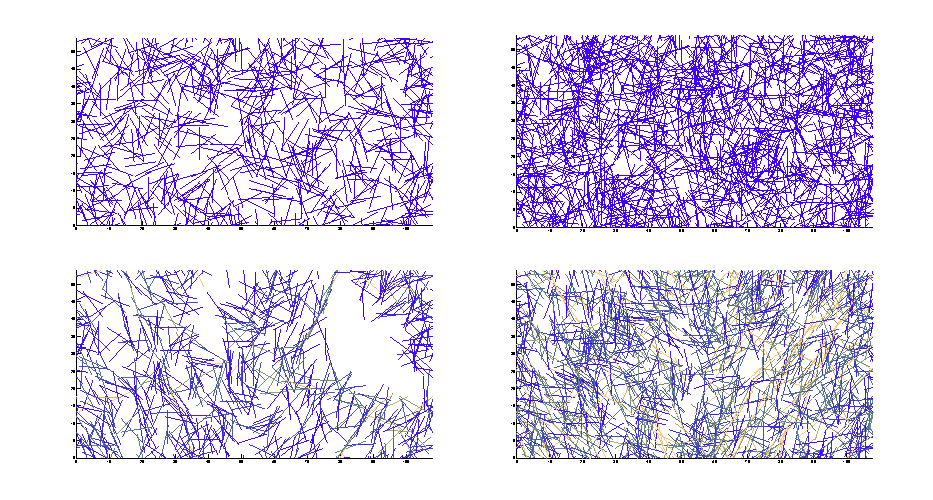
\includegraphics[width=\hsize]{network_def}
\caption{\label{fig:sim}Two Simulation setups with $L=9 \mu m, D = 54 \mu m$ before (top) and after  (bottom) 1000 seconds of applied stress. a) low density $l_c=2 \mu m$, b) moderate density $l_c=1 \mu m.  $ Scale bar $ 20 \mu m$}
\end{figure}

The nominal units for length, force, and time are $\mu m$, nN, and s, respectively.  We explored parameter space around an estimate of biologically relevant parameter values, given in Table \ref{table:para}. 

\begin{table}[h]
\centering
\caption{Simulation Parameter Values}
\label{table:para}
\begin{tabular}{|c|c|c|c|c|}
\hline
{\bf parameter}             & {\bf symbol} & {\bf physiological estimate}          \\ \hline
extensional modulus         & $\mu$        & $1 nN $                                               \\
bending modulus             & $\kappa$     & $ 10^{-3} nN \cdot \mu m$                           \\
cross-link drag coefficient & $\xi$      & $unknown $              \\
medium drag coefficient     & $\zeta$        & $0.0005 \frac{nN s}{\mu m^2} $      \\
filament length             & L            & $5 \mu m$                                          \\
cross-link spacing          & $l_c$        & $0.5 \mu m$                                         \\
domain size                 & D            & $10-50 \mu m$                                 \\ \hline
\end{tabular}
\end{table}



% Results and Discussion can be combined.
\section*{Results and Discussion}













\section*{Supporting Information}

% Include only the SI item label in the subsection heading. Use the \nameref{label} command to cite SI items in the text.
\subsection*{S1 Video}
\label{S1_Video}
{\bf Bold the first sentence.}  Maecenas convallis mauris sit amet sem ultrices gravida. Etiam eget sapien nibh. Sed ac ipsum eget enim egestas ullamcorper nec euismod ligula. Curabitur fringilla pulvinar lectus consectetur pellentesque.

\subsection*{S1 Text}
\label{S1_Text}
{\bf Lorem Ipsum.} Maecenas convallis mauris sit amet sem ultrices gravida. Etiam eget sapien nibh. Sed ac ipsum eget enim egestas ullamcorper nec euismod ligula. Curabitur fringilla pulvinar lectus consectetur pellentesque.

\subsection*{S1 Fig}
\label{S1_Fig}
{\bf Lorem Ipsum.} Maecenas convallis mauris sit amet sem ultrices gravida. Etiam eget sapien nibh. Sed ac ipsum eget enim egestas ullamcorper nec euismod ligula. Curabitur fringilla pulvinar lectus consectetur pellentesque.

\subsection*{S2 Fig}
\label{S2_Fig}
{\bf Lorem Ipsum.} Maecenas convallis mauris sit amet sem ultrices gravida. Etiam eget sapien nibh. Sed ac ipsum eget enim egestas ullamcorper nec euismod ligula. Curabitur fringilla pulvinar lectus consectetur pellentesque.

\subsection*{S1 Table}
\label{S1_Table}
{\bf Lorem Ipsum.} Maecenas convallis mauris sit amet sem ultrices gravida. Etiam eget sapien nibh. Sed ac ipsum eget enim egestas ullamcorper nec euismod ligula. Curabitur fringilla pulvinar lectus consectetur pellentesque.

\section*{Acknowledgments}
Cras egestas velit mauris, eu mollis turpis pellentesque sit amet. Interdum et malesuada fames ac ante ipsum primis in faucibus. Nam id pretium nisi. Sed ac quam id nisi malesuada congue. Sed interdum aliquet augue, at pellentesque quam rhoncus vitae.

\nolinenumbers

%\section*{References}
% Either type in your references using
% \begin{thebibliography}{}
% \bibitem{}
% Text
% \end{thebibliography}
%
% OR
%
% Compile your BiBTeX database using our plos2015.bst
% style file and paste the contents of your .bbl file
% here.
% 
\bibliographystyle{plos2015}
\bibliography{slippage,active}

\begin{comment}
\begin{thebibliography}{10}
\bibitem{bib1}
Devaraju P, Gulati R, Antony PT, Mithun CB, Negi VS. Susceptibility to SLE in South Indian Tamils may be influenced by genetic selection pressure on TLR2 and TLR9 genes. Mol Immunol. 2014 Nov 22. pii: S0161-5890(14)00313-7. doi: 10.1016/j.molimm.2014.11.005

\bibitem{bib2}
Huynen MMTE, Martens P, Hilderlink HBM. The health impacts of globalisation: a conceptual framework. Global Health. 2005;1: 14. Available: http://www.globalizationandhealth.com/content/1/1/14.

\end{thebibliography}
\end{comment}


\end{document}

